%
% einleitung.tex -- Beispiel-File für die Einleitung
%
% (c) 2020 Prof Dr Andreas Müller, Hochschule Rapperswil
%
% !TEX root = ../../buch.tex
% !TEX encoding = UTF-8
%
\section{Differentialgleichung für Geodätenlinien
\label{geodaeten:section:Standardverfahren}}
\rhead{Differentialgleichung für Geodätenlinien}

Die Länge einer Kurve auf einer Ebene mit kartesischen Koordinaten lässt sich durch das Integral
\begin{equation}
	L = \int_{x_1}^{x_2} \sqrt{1 + \left(y'\right)^2} \, dx
\end{equation}
berechnen.
Um den kürzesten Abstand zwischen beiden Punkten zu finden, minimiert man dieses Längenintegral.
Man identifiziert zuerst die Lagrange-Funktion
\begin{equation}
	\mathcal{L}(y, y') = \sqrt{1 + \left(y'\right)^2},
\end{equation}
und bildet daraus die Euler-Lagrange-Differentialgleichung
\begin{equation}
	\frac{d}{dx} \left(\frac{\partial \mathcal{L}}{\partial y'}\right) - \frac{\partial \mathcal{L}}{\partial y} = 0.
\end{equation}
Durch Umformungen und Vereinfachungen ergibt sich letztendlich eine Differentialgleichung in der Form
\begin{equation}
	0 = \frac{y''}{\left(1 + \left(y'\right)^2\right)^{\frac{3}{2}}},
\end{equation}
deren Lösung eine Funktion beschreibt, die den kürzesten Abstand zwischen zwei Punkten auf einer Ebene darstellt. Wie wir später sehen werden, ist die Lösung dieser Gleichung eine Gerade, was intuitiv einleuchtend ist.

Nun stellen wir uns die Frage, ob wir mit unserem neu erlernten Wissen eine allgemeine Differentialgleichung finden können, welche die Funktion des kürzesten Abstands zwischen zwei Punkten für beliebige $n$-dimensionale geometrische Räume beschreibt.

\subsection{Formulierung des Variationsprinzips}
Wir beginnen mit dem allgemeinen Linienelement
\begin{equation}
	ds^2 = g_{ij} \, du^i \, du^j.
\end{equation}
Dieses parametrisieren wir nun nach einem gemeinsamen Parameter, wie zum Beispiel der Zeit, und erhalten
\begin{equation}
	ds^2 = g_{ij} \, \dot{u}^i \dot{u}^j \, dt^2,
\end{equation}
wobei $\dot{u}^i = \frac{du^i}{dt}$ die Ableitungen der Koordinaten nach der Zeit $t$ darstellen.

Durch die gemeinsame Parametrisierung lässt sich nun das Funktional für die Variation
\begin{equation}
	L = \int_{t_1}^{t_2} \sqrt{g_{ij} \, \dot{u}^i \dot{u}^j} \, dt
	\label{geodaeten:equation:StandardverfahrenGeodaeten:Funktional}
\end{equation}
als Integral des zu minimierenden Weges aufstellen.
Die Verwendung des raumspezifischen metrischen Tensors ermöglicht es, diese allgemeine Formel für jede Art von Raum anzuwenden.

Weil das Funktional nur von einem einzigen Parameter abhängt, können wir die klassische Euler-Lagrange-Differentialgleichung verwenden.
Als erstes identifizieren wir somit die Lagrange-Funktion als
\begin{equation}
	\mathcal{L}(u^n, \dot{u}^n) = \sqrt{g_{ij} \, \dot{u}^i \dot{u}^j}.
	\label{geodaeten:equation:StandardverfahrenGeodaeten:LagrangeFunktion}
\end{equation}

Da das Funktional eine $n$-dimensionale Anzahl an Koordinaten umfasst, die selbst Funktionen des Parameters $t$ sind, muss für jede Koordinate eine Euler-Lagrange-Differentialgleichung in der Form von
\begin{equation}
	\frac{d}{dt} \left(\frac{\partial \mathcal{L}}{\partial \dot{u}^n}\right) - \frac{\partial \mathcal{L}}{\partial u^n} = 0
	\label{geodaeten:equation:StandardverfahrenGeodaeten:DGL1}
\end{equation}
aufgestellt werden.
Für einen $n$-dimensionalen Raum ergeben sich somit auch $n$ Differentialgleichungen. 

\subsection{Vereinfachungen und Rahmenbedingungen}
Wir setzen voraus, dass der Radikand des Funktionals \eqref{geodaeten:equation:StandardverfahrenGeodaeten:Funktional} nicht negativ wird, die Koordinaten sowie ihre Ableitungen stetig sind, und dass ein differenzierbarer metrischer Tensor existiert. 
Diese Voraussetzungen charakterisieren eine Riemannsche Mannigfaltigkeit.
Daher gilt diese Variationsrechnung für beliebige geometrische Räume unter der Voraussetzung, dass sie als Riemannsche Mannigfaltigkeiten interpretiert werden können\footnote{Tatsächlich gelten die Geodätengleichungen, die sich aus dieser Variationsrechnung ergeben, auch für sogenannte Pseudo-Riemannsche Räume.
	In diesen Räumen kann die Metrik negative Werte annehmen, wie es für die Beschreibung gekrümmter Raumzeiten der Fall ist.
	Die Herleitung weicht zwar leicht ab, aber das Ergebnis, die allgemeine Geodätengleichung, bleibt gleich.
}.

Um weitere Berechnungen zu vereinfachen, substituieren wir den Radikanden in \eqref{geodaeten:equation:StandardverfahrenGeodaeten:LagrangeFunktion} mit
\begin{equation}
	\varphi = g_{ij} \, \dot{u}^i \dot{u}^j.
	\label{geodaeten:equation:StandardverfahrenGeodaeten:Substitution}
\end{equation}
Damit ergibt sich die Euler-Lagrange-Differentialgleichung \eqref{geodaeten:equation:StandardverfahrenGeodaeten:DGL1} zu
\begin{equation}
	\frac{d}{dt} \left(\frac{1}{2 \sqrt{\varphi}} \, \varphi_{\dot{u}^n}\right) - \frac{1}{2 \sqrt{\varphi}} \, \varphi_{u^n} = 0,
	\label{geodaeten:equation:StandardverfahrenGeodaeten:DGL2}
\end{equation}
wobei $\varphi_{\dot{u}^n} = \frac{\partial \varphi}{\partial \dot{u}^n}$ und $\varphi_{u^n} = \frac{\partial \varphi}{\partial u^n}$ die partiellen Ableitungen von $\varphi$ nach den jeweiligen Koordinaten sind.

Wir nehmen zusätzlich an, dass $\varphi = 1$ ist.
Daraus folgt gemäss \eqref{geodaeten:equation:StandardverfahrenGeodaeten:Funktional}, dass der Parameter $t$ mit der Bogenlänge $s$ identifiziert werden kann und daher als natürlicher Parameter fungiert. 
Diese Annahme ist gerechtfertigt, da der Ausdruck für $\varphi$ dem Quadrat des tangentialen Geschwindigkeitsvektors entspricht und die Geschwindigkeit, mit der die Geodäte durchlaufen wird, die Form der Geodäte selbst nicht verändert.
Dadurch vereinfacht sich die Gleichung \eqref{geodaeten:equation:StandardverfahrenGeodaeten:DGL2} noch weiter zu
\begin{equation}
	\frac{d}{ds} \left( \varphi_{\dot{u}^n} \right) - \varphi_{u^n} = 0,
	\label{geodaeten:equation:StandardverfahrenGeodaeten:DGL3}
\end{equation}
wobei die Punktableitungen hier bedeuten, dass jetzt nach $s$ abgeleitet wird.

\subsection{Berechnung der Ableitungen}
Für die partielle Ableitung $\varphi_{u^n}$ erhalten wir
\begin{equation} 
	\frac{\partial \varphi}{\partial u^n} = \frac{\partial}{\partial u^n} \left(g_{ij} \, \dot{u}^i \, \dot{u}^j\right) = \frac{\partial \, g_{ij}}{\partial u^n} \, \dot{u}^i \, \dot{u}^j. 
	\label{geodaeten:equation:StandardverfahrenGeodaeten:PartialPhi1}
\end{equation}

Die partielle Ableitung $\varphi_{\dot{u}^n}$ ergibt sich aus
\begin{equation}
	\frac{\partial \varphi}{\partial \dot{u}^n} = g_{ij} \, \frac{\partial}{\partial \dot{u}^n} \left( \dot{u}^i \dot{u}^j \right),
\end{equation}
wobei es zwei Fälle zu betrachten gibt, abhängig davon, ob $i = n$ oder $j = n$:
\begin{itemize}
	\item Wenn $i = n$, dann ist $\frac{\partial \dot{u}^i}{\partial \dot{u}^n} = 1$ und $\frac{\partial \dot{u}^j}{\partial \dot{u}^n} = 0$, für $i \neq j$.
	\item Wenn $j = n$, dann ist $\frac{\partial \dot{u}^j}{\partial \dot{u}^n} = 1$ und $\frac{\partial \dot{u}^i}{\partial \dot{u}^n} = 0$, für $i \neq j$.
\end{itemize}
Aus der Produktregel ergibt sich somit
\begin{equation}
	\frac{\partial \varphi}{\partial \dot{u}^n} = g_{nj} \dot{u}^j + g_{in} \dot{u}^i,
\end{equation}
und weil $g_{ij}$ symmetrisch ist ($g_{ij} = g_{ji}$), lässt sich dies zusammenfassen zu
\begin{equation}
	\frac{\partial \varphi}{\partial \dot{u}^n} = 2g_{in} \dot{u}^i.
	\label{geodaeten:equation:StandardverfahrenGeodaeten:PartialPhi2}
\end{equation}

Da $\varphi_{\dot{u}^n}$ von den Koordinaten $u^k$ und deren Ableitungen $\dot{u}^k$ abhängt, berechnet sich die Ableitung von $\varphi_{\dot{u}^n}$ nach $s$ durch Anwendung der Kettenregel als
\begin{equation}
	\frac{d}{ds} \left( \varphi_{\dot{u}^n} \right) = \sum_{k = 1}^n \left( \frac{\partial \varphi_{\dot{u}^n}}{\partial u^k} \, \dot{u}^k + \frac{\partial \varphi_{\dot{u}^n}}{\partial \dot{u}^k} \, \ddot{u}^k \right),
	\label{geodaeten:equation:StandardverfahrenGeodaeten:Ableitung1s}
\end{equation}
wobei ab diesem Punkt die Summierung über den Index $k$ implizit erfolgt, wie es beim metrischen Tensor üblich ist.

Mithilfe von \eqref{geodaeten:equation:StandardverfahrenGeodaeten:PartialPhi2} erhalten wir für die partielle Ableitung nach $u^k$  
\begin{equation}
	\frac{\partial \varphi_{\dot{u}^n}}{\partial u^k} = 
	2 \frac{\partial g_{in}}{\partial u^k} \ \dot{u}^i
\end{equation}
und für die Ableitung nach $\dot{u}^k$
\begin{equation}
	\frac{\partial \varphi_{\dot{u}^n}}{\partial \dot{u}^k} = 
	2 \, g_{kn}.
\end{equation}

Daraus folgt schliesslich für \eqref{geodaeten:equation:StandardverfahrenGeodaeten:Ableitung1s}
\begin{equation}
	\frac{d}{ds} \left( \varphi_{\dot{u}^n} \right) = 2 \frac{\partial g_{in}}{\partial u^k} \ \dot{u}^i \dot{u}^k + 2 g_{kn} \, \ddot{u}^k.
	\label{geodaeten:equation:StandardverfahrenGeodaeten:Ableitung2s}
\end{equation}

\subsection{Formulierung der allgemeinen Geodätengleichung}
Fügt man nun alles zusammen und setzt \eqref{geodaeten:equation:StandardverfahrenGeodaeten:PartialPhi1} und \eqref{geodaeten:equation:StandardverfahrenGeodaeten:Ableitung2s} in die Gleichung \eqref{geodaeten:equation:StandardverfahrenGeodaeten:DGL3} ein, ergibt sich
\begin{equation}
	2 \frac{\partial g_{in}}{\partial u^k} \ \dot{u}^i \dot{u}^k + 2 g_{kn} \, \ddot{u}^k - \frac{\partial g_{ij}}{\partial u^n} \, \dot{u}^i \, \dot{u}^j = 0.
\end{equation}

Im ersten Summanden tritt jedoch ein Problem auf, da dieser Term nicht symmetrisch ist. 
Die Koeffizienten $\frac{\partial g_{in}}{\partial u^k}$ und $\frac{\partial g_{kn}}{\partial u^i}$ können unterschiedlich sein, was die symmetrische Eigenschaft des metrischen Tensors gefährdet. 
Um dies zu korrigieren, bildet man den Mittelwert der beiden Koeffizienten
\begin{equation}
	\frac{1}{2} \left( \frac{\partial g_{kn}}{\partial u^i} + \frac{\partial g_{in}}{\partial u^k} \right),
\end{equation}
wodurch sich die Symmetrie wiederherstellen lässt.

Der korrigierte Ausdruck lautet dann
\begin{equation}
	2 \cdot \frac{1}{2} \left( \frac{\partial g_{kn}}{\partial u^i} + \frac{\partial g_{in}}{\partial u^k} \right) \dot{u}^i \dot{u}^k + 2 g_{kn} \, \ddot{u}^k - \frac{\partial g_{ij}}{\partial u^n} \, \dot{u}^i \, \dot{u}^j = 0.
\end{equation}

Da der Index $k$ im ersten Summanden und der Index $j$ im letzten Summanden beide bis $n$ summiert werden, kann der Index $k$ durch $j$ ersetzt werden. 
Dadurch lässt sich der Term $g_{ij}$ aufgrund der wiederhergestellten Symmetrie teilweise ausklammern und es ergibt sich
\begin{equation}
	2 g_{kn} \, \ddot{u}^k + \left( \frac{\partial g_{jn}}{\partial u^i} + \frac{\partial g_{in}}{\partial u^j} - \frac{\partial g_{ij}}{\partial u^n} \right) \, \dot{u}^i \, \dot{u}^j = 0.
\end{equation}
Multipliziert man den gesamten Ausdruck mit $\frac{1}{2} g^{kn}$ und benennt den Index $n$ in $l$ um, so erhält man die Gleichung
\begin{equation}
	\ddot{u}^k + \frac{1}{2} g^{kl} \left( \frac{\partial g_{jl}}{\partial u^i} + \frac{\partial g_{il}}{\partial u^j} - \frac{\partial g_{ij}}{\partial u^l} \right) \dot{u}^i \dot{u}^j = 0,
\end{equation}
wobei $g^{kl}$ die Inverse des metrischen Tensors darstellt.

Dieser Ausdruck kann durch die sogenannten Christoffel-Symbole $\Gamma^k_{ij}$ weiter zusammengefasst werden.
Diese sind definiert als
\begin{equation}
	\Gamma^k_{ij} = \frac{1}{2} g^{kl} \left( \frac{\partial g_{jl}}{\partial u^i} + \frac{\partial g_{il}}{\partial u^j} - \frac{\partial g_{ij}}{\partial u^l} \right),
	\label{geodaeten:equation:StandardverfahrenGeodaeten:ChristopherSymbole}
\end{equation}
und sind aufgrund der wiederhergestellten Symmetrie des metrischen Tensors, ebenfalls in den Indizes $i$ und $j$ symmetrisch ($\Gamma^k_{ij} = \Gamma^k_{ji}$).

Durch die Einführung der Christoffel-Symbole erhält man so schliesslich die allgemeine Geodätengleichung
\begin{equation}
	\ddot{u}^k + \Gamma^k_{ij} \dot{u}^i \dot{u}^j = 0.
	\label{geodaeten:equation:StandardverfahrenGeodaeten:Geodaetengleichung}
\end{equation}

Diese allgemeine Geodätengleichung kann so interpretiert werden, dass der kürzeste Weg zwischen zwei Punkten prinzipiell immer eine Gerade ist. 
Allerdings wird die Vorstellung einer Geraden durch die Geometrie des Raumes verzerrt und nimmt je nach Raum eine andere Form an. 
Hier kommen die Christoffel-Symbole in der Geodätengleichung ins Spiel.

Die Christoffel-Symbole beschreiben, wie sich ein Raum in die Richtung einer Dimension ändert.
Sie wirken wie Wegweiser, welche die Geodäten so korrigieren, dass sie im jeweiligen Raum am geradlinigsten verlaufen. 
Da die Christoffel-Symbole von der Geometrie des Raumes abhängen, reflektieren sie auch die Krümmung des Raumes.
Wenn beispielsweise alle Christoffel-Symbole null sind, ist der Raum krümmungsfrei, und eine Gerade bleibt eine Gerade.

Mit dieser allgemeinen Geodätengleichung können nun die Geodätenlinien für beliebige $n$-dimensionale Räume berechnet werden. 
Anstatt das Variationsprinzip jedes Mal von Grund auf anzuwenden, kann die Geodätengleichung direkt genutzt werden, um daraus standardmässig die Funktion des kürzesten Weges zu ermitteln (Abschnitt \ref{geodaeten:section:StandardverfahrenBeispiele}).

\section{Beispiele zu den Differentialgleichungen für Geodätenlinien 
\label{geodaeten:section:StandardverfahrenBeispiele}}

%
% einleitung.tex -- Beispiel-File für die Einleitung
%
% (c) 2020 Prof Dr Andreas Müller, Hochschule Rapperswil
%
% !TEX root = ../../buch.tex
% !TEX encoding = UTF-8
%
\subsection{Kartesisch\label{geodaeten:section:Standardverfahren:Kartesisch}}
\rhead{Standardverfahren Beispiele}

Für den kartesischen Raum mit dem metrischen Tensor
\begin{equation}
g_{ij} = \begin{pmatrix} 
	1 & 0 \\ 
	0 & 1 
\end{pmatrix},
\end{equation}
wollen wir die Christoffel-Symbole \eqref{geodaeten:equation:StandardverfahrenGeodaeten:ChristopherSymbole} berechnen.

Da der metrische Tensor $g_{ij}$ konstant ist und keine direkte Abhängigkeit von den Koordinaten aufweist, verschwinden alle Ableitungen.
Ohne weitere Berechnungen kann man also schliessen, dass
\begin{equation}
\frac{\partial g_{ij}}{\partial u^k} = 0 .
\end{equation}
Somit ergeben sich alle Christoffel-Symbole zu
\begin{equation}
\Gamma^i_{jk} = 0 .
\end{equation}

Denkt man an die Definition aus Abschnitt \ref{geodaeten:section:Standardverfahren}, macht dies durchaus Sinn.
Denn der Kartesische Raum ist nicht gekrümmt, weshalb keine Korrektur der Geraden notwendig ist.

Setzt man die Christoffel-Symbole in die allgemeine Geodätengleichung \eqref{geodaeten:equation:StandardverfahrenGeodaeten:Geodaetengleichung} ein, erhält man mit $u^1 = x(t)$
\begin{equation}
	\begin{alignedat}{3}
		&\ddot{u}^1 + \Gamma_{ij}^1 \dot{u}^i \dot{u}^j &\quad = \quad& 0 \\
		% &\ddot{u}^1 + 0_{ij} \cdot \dot{u}^i \dot{u}^j &\quad = \quad& 0\\
		%&\ddot{u}^1  &\quad = \quad& 0 \\
		&\ddot{x}(t) &\quad = \quad& 0
	\end{alignedat}
	\label{geodaeten:equation:Standardverfahren:Kartesisch:x}
\end{equation}
und mit $u^2 = y(t)$
\begin{equation}
	\begin{alignedat}{3}
		&\ddot{u}^2 + \Gamma_{ij}^2 \dot{u}^i \dot{u}^j &\quad = \quad& 0 \\
		% &\ddot{u}^2 + 0_{ij} \cdot \dot{u}^i \dot{u}^j &\quad = \quad& 0 \\
		% &\ddot{u}^2  &\quad = \quad& 0 \\
		&\ddot{y}(t) &\quad = \quad& 0  .
	\end{alignedat}
	\label{geodaeten:equation:Standardverfahren:Kartesisch:y}
\end{equation}

Da die zweite Ableitung in beiden Dimensionen Null ist, erkennt man bereits, dass es sich beim kürzesten Weg um eine Gerade handeln muss, was aus Erfahrung durchaus sinnvoll erscheint.

Setzt man nun zwei Punkte als Start und Endpunkt, kann man durch diese Nebenbedingungen eine konkrete Lösung erhalten.
Als Beispiel möchten wir den kürzesten Weg zwischen den Punkten $P_A = (1,1)$ und $P_B = (3,5)$ berechnen. 
Durch doppeltes Integrieren der Gleichung \eqref{geodaeten:equation:Standardverfahren:Kartesisch:x} erhält man
\begin{equation}
	\frac{d^2x}{dt^2} = 0 
	\Rightarrow \frac{dx}{dt} = c_1 
	\Rightarrow x(t) = c_1 \cdot t + c_2  .
	\label{geodaeten:equation:Standardverfahren:Kartesisch:equation1}
\end{equation}
Dabei sind $c_1$  und $c_2$ Integrationskonstanten. 

Wir sehen, die Gleichung entspricht einer parametrierten Geradengleichung mit $c_2$ als Startwert für $x(0)$ und $c_1$ als Steigung von $x(t)$. 
Mit $P_A(x_1,y_1)$ und $P_B(x_2,y_2)$ haben diese Gleichungen die Form
\begin{align}
	x(t) &= (x_2 - x_1) \cdot t + x_1 \\
	y(t) &= (y_2 - y_1) \cdot t + y_1 .
\end{align}
Da die Gerade durch den Startpunkt gehen muss ist der Startwert bei $t=0$ gegeben durch
\begin{equation}
	0 \cdot c_1 + c_2 = 1 \Rightarrow c_2 = 1 .	
\end{equation}
Die Steigung $c_1$ kann mithilfe von Endpunkt und Startpunkt berechnet werden als
\begin{equation}
	c_1 = x_2 - x_1 \\ = 3-1 \\ = 2
\end{equation}
und damit ist die Lösung der Geodätengleichung in $x$ gleich
\begin{equation}
	x(t) = 2t + 1 .
	\label{geodaeten:equation:StaKartesisch:LoesungX}
\end{equation}

Analog für $y(t)$ ergibt sich die Lösung der Geodätengleichung in $y$ zu
\begin{equation}
	y(t) = 4t + 1 .
	\label{geodaeten:equation:StaKartesisch:LoesungY}
\end{equation}
Die resultierende Kurve ist in Abbildung \ref{geodaeten:figure:Standardverfahren:Kartesisch:figure1} dargestellt.
\begin{figure}
	\centering
	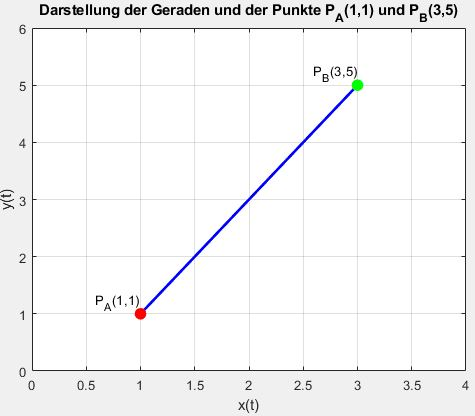
\includegraphics[width=10cm]{papers/geodaeten/Abbildungen/Standardverfahren/Kartesisch}
	\label{geodaeten:figure:Standardverfahren:Kartesisch:figure1}
	\caption{Darstellung der Kurve von x(t) und y(t) mit $t \in [0 , 1]$ Wie man sieht ist der kürzeste Weg von Punkt A zu Punkt B eine gerade.}
\end{figure}

%
% einleitung.tex -- Beispiel-File für die Einleitung
%
% (c) 2020 Prof Dr Andreas Müller, Hochschule Rapperswil
%
% !TEX root = ../../buch.tex
% !TEX encoding = UTF-8
%
\subsection{Zylinder\label{geodaeten:section:Standardverfahren:Zylinder}}
\rhead{Standardverfahren Beispiele}

Für die Zylinderoberfläche mit konstantem $r$ und dem metrischen Tensor 
\begin{equation}
	g_{ij} = \begin{pmatrix} 
		r^2 & 0 \\ 
		0 & 1 
	\end{pmatrix}
\end{equation}
wollen wir die Christoffel-Symbol berechnen. 
Wie bei dem kartesischen Raum (Abschnitt \ref{geodaeten:section:Standardverfahren:Kartesisch}) werden alle Christoffel-Symbol Null, da der metrische Tensor konstant ist\footnote{
Auch in diesem Beispiel sind die Christoffel-Symbol gleich Null.
Auf den ersten Blick könnte das verwirrend sein, da man bei einem Zylinder doch eindeutig eine Krümmung sieht.
Der Grund dafür ist, dass es sich bei dem Zylinder um eine extrinsische Krümmung handelt.
Die Zylinderoberfläche wird von aussen zu einem Zylinder gekrümmt.
Abgerollt sieht man allerdings, dass die Oberfläche flach ist.
Als weiteres Beispiel lässt sich berechnen, dass die Christoffel-Symbol im Polarkoordinaten-Raum nicht gleich Null sind und daher eine Krümmung existiert, obwohl der Raum flach erscheint.
Damit zeigt sich, dass die Intuition in diesem Fall täuschen kann.
}.
Wir ersparen uns hier deshalb diese Rechnung.

Setzt man $u^1 = \phi (t)$ und $u^2 = z(t)$ in die Geodätengleichung ein, so erhält man analog zu \eqref{geodaeten:equation:Standardverfahren:Kartesisch:x}
\begin{equation}
	\ddot{\phi}(t) = 0
	\label{geodaeten:equation:Standardverfahren:Zylinder:phi}
\end{equation}
und dementsprechend gemäss \eqref{geodaeten:equation:Standardverfahren:Kartesisch:y}
\begin{equation}
	\ddot{z}(t) = 0 .
\end{equation}


Wählen wir $P_A(\phi_1 , z_1) = P_A(1 , 1)$ und $P_B(\phi_2 , z_2) = P_B(3 , 5)$ gleich wie in Abschnitt \ref{geodaeten:section:Standardverfahren:Kartesisch}, kennen wie bereits die Lösungen. 
Aus \eqref{geodaeten:equation:StaKartesisch:LoesungX} wird 
\begin{equation}
	\phi(t) = 2t + 1 ,
\end{equation}
und aus \eqref{geodaeten:equation:StaKartesisch:LoesungY} wird
\begin{equation}
	z(t) = 4t + 1 .
\end{equation}

Beim Zylinder ist jedoch interessant, dass es beliebig viele weitere Lösungen für die Geodätengleichung gibt, da Die Winkelkoordinate periodisch ist.
Durch Hinzufügen eines Vielfachen von $2\pi$ macht die Kurve zusätzliche Runden um den Zylinder, bevor sie auf den Punkt $P_B$ trifft, wie in Abbildung \ref{geodaeten:figure:Standardverfahren:Zylinder:figure1} dargestellt.
Dies ist zwar nicht die kürzeste Strecke, jedoch wird weder die Gleichung \eqref{geodaeten:equation:Standardverfahren:Zylinder:phi} verletzt noch der Punkt $P_A$ oder $P_B$ verfehlt.
Deshalb existieren sie als Scheinlösungen der Geodätengleichung.

Wird die Oberfläche des Zylinders wie in Abbildung \ref{geodaeten:figure:Standardverfahren:Zylinder:figure1} auf eine Fläche abgerollt, ist ersichtlich, wie auch hier der kürzeste Weg eine Gerade ist.  

\begin{figure}
	\centering
	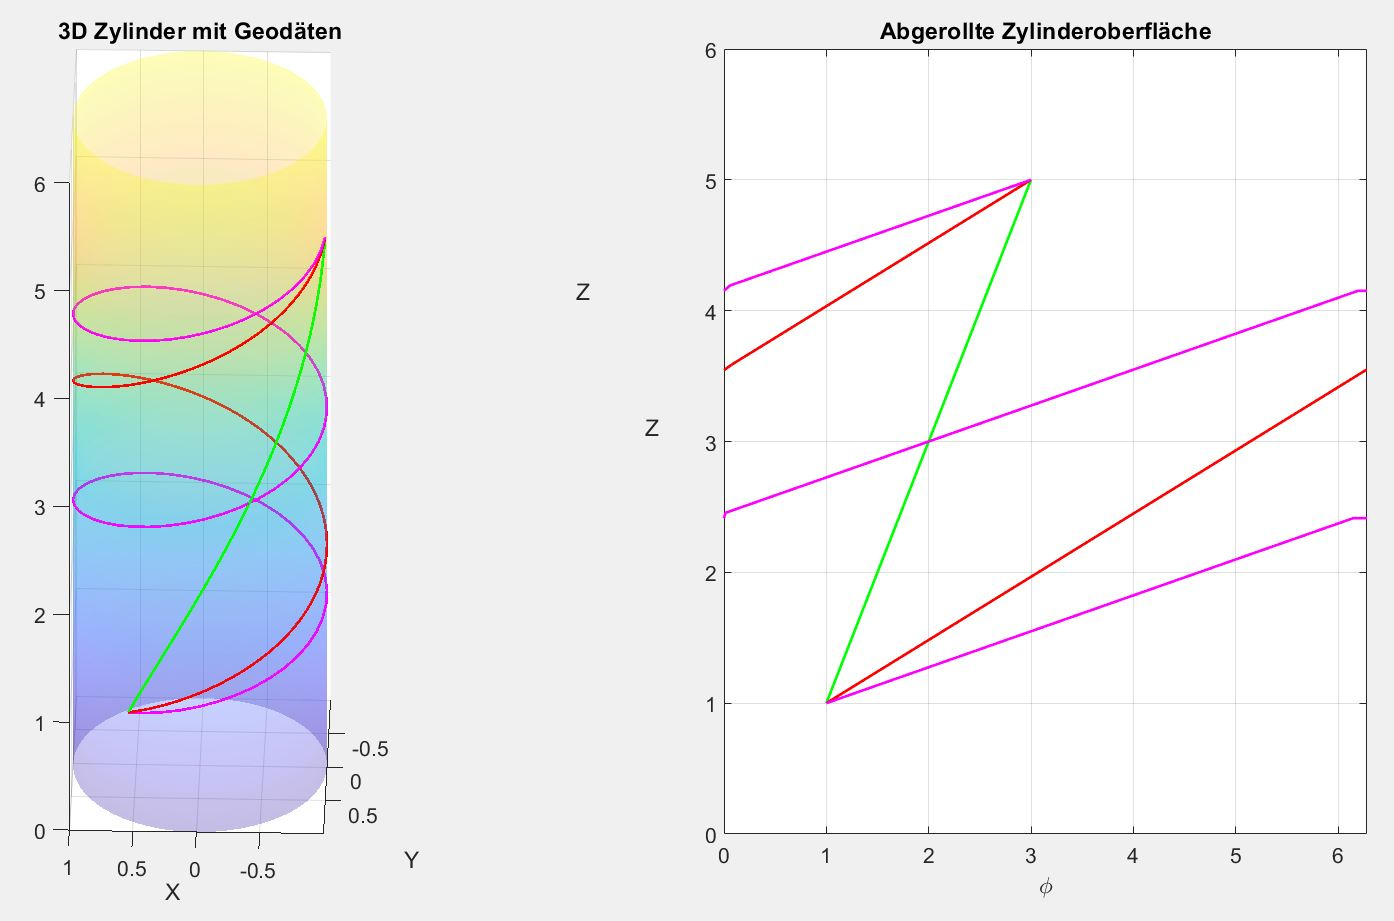
\includegraphics[width=\textwidth]{papers/geodaeten/Abbildungen/Standardverfahren/Zylinder}
	\caption{Darstellung der Geodätenlinien auf einem Zylinder und dessen abgerollte Oberfläche in einem 2D Plot mit Matlab.}
	\label{geodaeten:figure:Standardverfahren:Zylinder:figure1}
\end{figure}

%
% einleitung.tex -- Beispiel-File für die Einleitung
%
% (c) 2020 Prof Dr Andreas Müller, Hochschule Rapperswil
%
% !TEX root = ../../buch.tex
% !TEX encoding = UTF-8
%
\subsection{Kugel\label{geodaeten:section:Standardverfahren:Kugel}}
\rhead{Standardverfahren Beispiele}

Intuitiv erwarten wir, dass die Geodäten auf der Kugeloberfläche Grosskreise sind.
Ein Grosskreis ist der geradlinigste Weg zwischen zwei Punkten auf einer Kugel.
Dies kann man sich vorstellen, indem man zwei Nadeln in eine Kugeloberfläche steckt und einen Faden um die beiden Nadeln spannt.
Der Faden wird immer entlang eines Grosskreises verlaufen.
Tatsächlich folgen Flugzeuge auf Langstreckenflügen dieser Logik und fliegen entlang von Grosskreisen, um die kürzeste Strecke zwischen zwei Punkten auf der Erde zurückzulegen.
Wir möchten nun überprüfen, ob wir mit dem Standardverfahren tatsächlich zu dieser Lösung kommen.

Um dies zu tun, benötigen wir den bereits im vorherigen Abschnitt hergeleiteten metrischen Tensor für die Kugeloberfläche.
Dieser ist in Kugelkoordinaten $(\theta, \phi)$ gegeben durch
\begin{equation}
	g_{ij} = r^2 \begin{pmatrix}
		1 & 0 \\
		0 & \sin^2\theta
	\end{pmatrix}.
\end{equation}

Zuerst berechnen wir die Inverse des metrischen Tensors, da diese für die Berechnung der Christoffel-Symbol benötigt wird.
Der inverse Tensor $g^{ij}$ ergibt sich zu
\begin{equation}
	g^{ij} = \frac{1}{r^2} 
	\begin{pmatrix}
		1 & 0 \\
		0 & \frac{1}{\sin^2\theta}
	\end{pmatrix}.
	\label{geodaeten:equation:StaKugel:TensorInverse}
\end{equation}

Nun berechnen wir die partiellen Ableitungen des metrischen Tensors $g_{ij}$ in Bezug auf die Koordinaten $\theta$ und $\phi$.
Da $g_{11} = r^2$ und $g_{22} = r^2 \sin^2\theta$, erhalten wir
\begin{equation}
	\frac{\partial g_{11}}{\partial \theta} = 0, \quad \frac{\partial g_{11}}{\partial \phi} = 0, \quad \frac{\partial g_{22}}{\partial \theta} = 2r^2 \sin\theta \cos\theta, \quad \frac{\partial g_{22}}{\partial \phi} = 0.
	\label{geodaeten:equation:StaKugel:Ableitungen}
\end{equation}

\subsection{Christoffel-Symbole}
Mit den Ableitungen \eqref{geodaeten:equation:StaKugel:Ableitungen} und dem inversen Tensor $g^{ij}$ \eqref{geodaeten:equation:StaKugel:TensorInverse} können wir nun die Christoffel-Symbole berechnen durch
\begin{equation}
	\Gamma_{ij}^k = \frac{1}{2} g^{kl} \left( \frac{\partial g_{jl}}{\partial u^i} + \frac{\partial g_{il}}{\partial u^j} - \frac{\partial g_{ij}}{\partial u^l} \right),
\end{equation}
wobei $u^1 = \theta$ und $u^2 = \phi$.

Nach Einsetzen der Werte und Vereinfachung erhalten wir folgende nicht-verschwindende Christoffel-Symbole
\begin{equation}
	\Gamma_{12}^2 = \Gamma_{21}^2 = \cot\theta \quad \text{und} \quad \Gamma_{22}^1 = -\sin\theta \cos\theta.
\end{equation}

Anders als im Fall des Zylinders, wo der metrische Tensor konstant war, führt die Abhängigkeit des metrischen Tensors von der Koordinate $\theta$ zu nicht-verschwindenden Christoffel-Symbolen, welche die intrinsische Krümmung der Kugeloberfläche beschreiben.

Um diese Krümmung zu verstehen, betrachten wir die Bewegung eines Tangentialvektors auf der Oberfläche in Bezug auf die Basisvektoren.

Wird die Komponente des Vektors entlang eines Breitenkreises verändert, also in $\phi$-Richtung, führt das zu keiner Änderung der Vektorrichtung, da das Bogenmass von $\phi$ entlang eines Breitenkreises konstant bleibt.
Diese Bewegung beeinflusst die allgemeine Richtung des Vektors also nicht, was auch im metrischen Tensor reflektiert wird, der keinerlei Abhängigkeit von $\phi$ aufweist.

Andererseits führt eine Veränderung der Komponente entlang eines Längengrades, also in $\theta$-Richtung, zu einer Veränderung der Vektorrichtung.
Dies liegt daran, dass das Bogenmass von $\phi$ mit $\theta$ variiert: 
Je näher man den Polen kommt, desto kürzer wird der Bogen für eine gegebene Änderung von $\theta$, was die Gesamtrichtung des Vektors beeinflusst. 
Damit der Tangentialvektor seine ursprüngliche Richtung beibehält, müsste die Bewegung in der $\phi$-Richtung zunehmend verringert werden, je näher man den Polen kommt.

Diese Richtungsänderung des Vektors ist eine direkte Folge der intrinsischen Krümmung der Kugeloberfläche.
Die nicht-verschwindenden Christoffel-Symbole beschreiben genau diese Krümmung und geben an, wie sich die Richtung eines Vektors bei seiner Bewegung entlang der Oberfläche verändert.

\subsection{Geodätengleichung}
Mit den berechneten Christoffel-Symbolen können wir nun die Geodätengleichungen für die Kugeloberfläche aufstellen.

Die allgemeine Form der Geodätengleichung lautet
\begin{equation}
	\ddot{u}^k + \Gamma^k_{ij} \dot{u}^i \dot{u}^j = 0,
\end{equation}
wobei $u^k$ die Koordinaten darstellen, in diesem Fall $\theta$ und $\phi$.

Setzen wir die entsprechenden Christoffel-Symbole und Koordinaten in die Gleichungen ein, erhalten wir
\begin{equation}
	\begin{aligned} 
		0 &= \ddot{\theta} + \Gamma^1_{11} \dot{\theta} \dot{\theta} + 2\Gamma^1_{12} \dot{\theta}\dot{\phi} + \Gamma^1_{22} \dot{\phi} \dot{\phi} \\
		0 &= \ddot{\phi} + \Gamma^2_{11} \dot{\theta} \dot{\theta} + 2\Gamma^2_{12} \dot{\theta}\dot{\phi} + \Gamma^2_{22} \dot{\phi} \dot{\phi},
	\end{aligned}
\end{equation}
und weil einige der Christoffel-Symbole Null sind, vereinfachen sich die Geodätengleichungen schliesslich zu
\begin{align}
	0 &= \ddot{\theta} - \sin\theta \cos\theta \, \dot{\phi}^2 \\
	0 &= \ddot{\phi} + 2 \cot\theta \, \dot{\theta} \dot{\phi}.
\end{align}

Da $r$ lediglich ein Skalierungsfaktor ist, kürzt es sich in den Geodätengleichungen heraus. 
Die Geometrie wird allein durch die Winkelabhängigkeit bestimmt, sodass der Radius keinen Einfluss auf die Form der Geodäten hat.

Das Lösen der Geodätengleichungen ist oft aufwendig und schwierig, was numerische Ansätze erforderlich macht. 
Daher überprüfen wir durch Analyse, ob Grosskreise diese tatsächlich erfüllen und als Lösungen gelten.

\subsection{Äquator}
Betrachten wir die Geodätengleichungen für konstantes $\theta$, also entlang eines Breitengrads.
Für konstantes $\theta$ gilt $\dot{\theta} = 0$ und $\ddot{\theta} = 0$.
Setzen wir dies in die erste Geodätengleichung ein, so erhalten wir:
\begin{equation}
	0 = -\sin\theta \cos\theta \, \dot{\phi}^2.
\end{equation}
Die zweite Geodätengleichung vereinfacht sich zu $0 = \ddot{\phi}$, was zeigt, dass $\phi(t)$ linear in der Zeit variiert.
Diese erste Geodätengleichung wird nur für $\theta = \frac{\pi}{2}$ erfüllt, das heisst, nur für den Äquator.
Für alle anderen Breitengrade mit $\theta \neq \frac{\pi}{2}$ muss $\dot{\phi}$ gleich null werden, was bedeutet, dass es keine Bewegung in der $\phi$-Richtung gibt und somit keine Geodäte vorliegt.
Der Äquator, als einziger Breitengrad, erfüllt daher die Geodätengleichungen und ist ein Grosskreis.

\begin{figure}
	\centering
	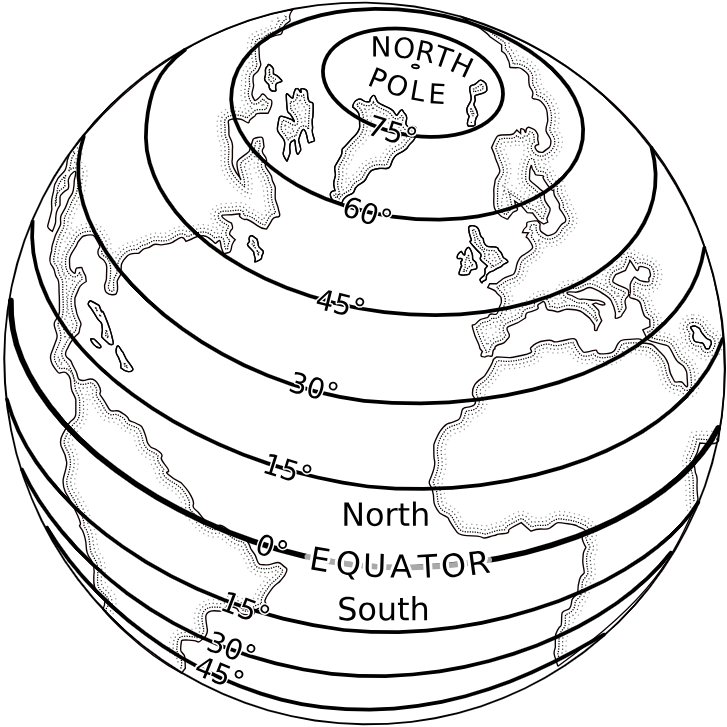
\includegraphics[width=7cm]{papers/geodaeten/Abbildungen/Standardverfahren/StaKugelBreitengrade}
	\caption{Erdkugel mit Breitengrade und Äquator als Geodätenlinie.}
	\label{geodaeten:figure:Standardverfahren:Breitengrade}
\end{figure}

\subsection{Längengrade}
Nun analysieren wir die Geodätengleichungen für konstantes $\phi$, also entlang eines Längengrads.
Für konstantes $\phi$ gilt $\dot{\phi} = 0$ und $\ddot{\phi} = 0$.
Setzen wir dies in die erste Geodätengleichung ein, erhalten wir:
\begin{equation}
	\ddot{\theta} = 0,
\end{equation}
was bedeutet, dass $\theta(t)$ linear in der Zeit variiert.
Die zweite Geodätengleichung wird ebenfalls trivial erfüllt, da $\dot{\phi} = 0$ und somit keine Beschleunigung in der $\phi$-Richtung vorliegt.
Damit sind alle Längengrade tatsächlich Geodäten.

Zusammenfassend konnten wir durch unsere Analyse zeigen, dass nur Grosskreise, wie der Äquator und die Längengrade, die Geodätengleichungen vollständig erfüllen und somit die wahren Geodäten auf der Kugeloberfläche darstellen.

Wir haben damit erfolgreich nachgewiesen, dass die Lösungen der Geodätengleichungen $\theta(t)$ und $\phi(t)$ zwangsläufig die Form von Grosskreisen annehmen müssen und dass die allgemeine Geodätengleichung diese Grosskreise korrekt als die Geodäten auf der Kugeloberfläche identifiziert.

\begin{figure}
	\centering
	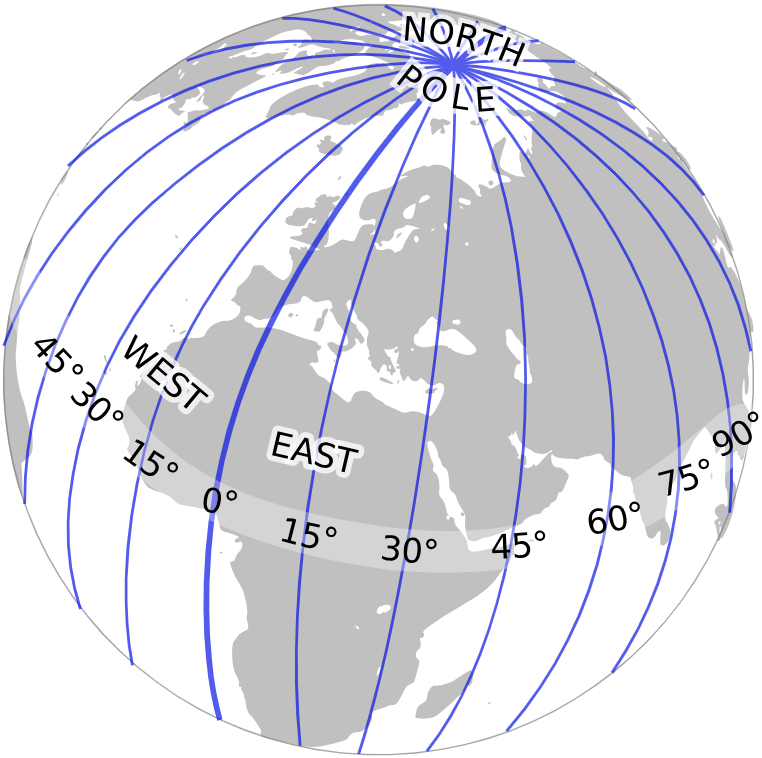
\includegraphics[width=7cm]{papers/geodaeten/Abbildungen/Standardverfahren/StaKugelLaengengrade}
	\caption{Erdkugel mit Längengrade als Geodätenlinen.}
	\label{geodaeten:figure:Standardverfahren:Laengengrade}
\end{figure}
